\documentclass{article}
\usepackage{fullpage}
\usepackage{multicol,multirow}
\usepackage{tabularx}
\usepackage{ulem}
\usepackage[utf8]{inputenc}
\usepackage[russian]{babel}
\usepackage{pgfplots}
\usepackage{graphicx}

\begin{document}

\section*{Лабораторная работа №5 по курсу «Численные методы»}

Выполнил студент группы М8О-408Б-20 Блинов Максим.
\\
Преподаватель: Пивоваров Д.\,Е.

\subsection*{Цель}

Используя явную и неявную конечно-разностные схемы, а также схему 
Кранка - Николсона, решить начально-краевую задачу для дифференциального 
уравнения параболического типа. Осуществить реализацию трех вариантов 
аппроксимации граничных условий, содержащих производные: двухточечная 
аппроксимация с первым порядком, трехточечная аппроксимация со вторым порядком, 
двухточечная аппроксимация со вторым порядком. В различные моменты времени 
вычислить погрешность численного решения путем сравнения результатов с 
приведенным в задании аналитическим решением $ U(x, t) $. Исследовать 
зависимость погрешности от сеточных параметров $ \tau, h $.

\subsection*{Вариант 3}
$$ \frac{\partial u}{\partial t} = a \frac{\partial^2 u}{\partial x^2}, \quad a > 0, $$
$$ u(0, t) = \exp(- at), $$
$$ u(\pi, t) = - \exp(- at), $$
$$ u(x, 0) = \cos x. $$

\text{Аналитическое решение: } $$ U(x, t) = \exp(- at) \cos x. $$


\subsection*{О программе}

Программа была реализована на языке программирования Go и включает в себя три численных метода для решения дифференциальных уравнений: 
явный метод (explicit), неявный метод (implicit) и метод Кранка-Николсона (Crank-Nicolson). Для визуализации результатов использовалась библиотека Gonum, 
которая предоставляет широкие возможности для построения графиков в среде Go. Результаты вычислений иллюстрируют поведение решений в зависимости от времени 
и начальных условий, а также позволяют оценить точность численных методов путём сравнения с аналитическим решением задачи. 
Графики ошибок демонстрируют различия между аналитическими и численными решениями на протяжении всего временного интервала. 
Все вычислительные эксперименты и генерация графиков проводились в рамках данной программы.

\subsection*{Инструкция к запуску}
Для запуска программы на Go, решающей гиперболические дифференциальные уравнения, убедитесь, что у вас установлена последняя версия Go 
(на данный момент 1.21, проверьте на официальном сайте). Создайте рабочее пространство, затем установите необходимые зависимости go mod tidy.

\pagebreak
\subsection*{Результаты}
\begin{center}
Полученные вычисления на момент времени $ t = 0.5 $
\\
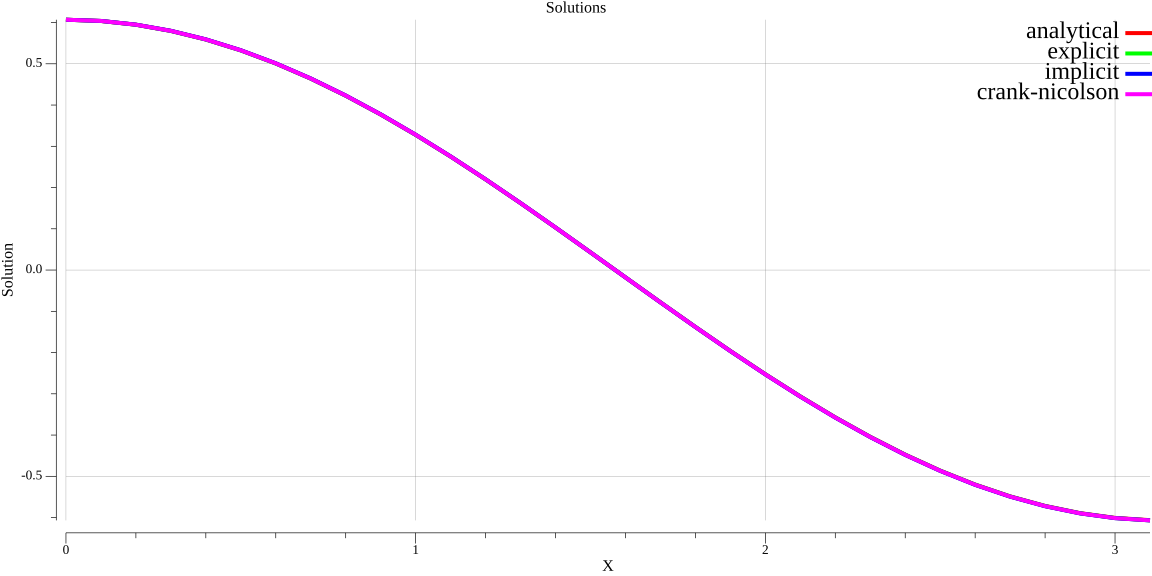
\includegraphics[scale=0.4]{solutions.png}
\\


Изменение погрешности
\\
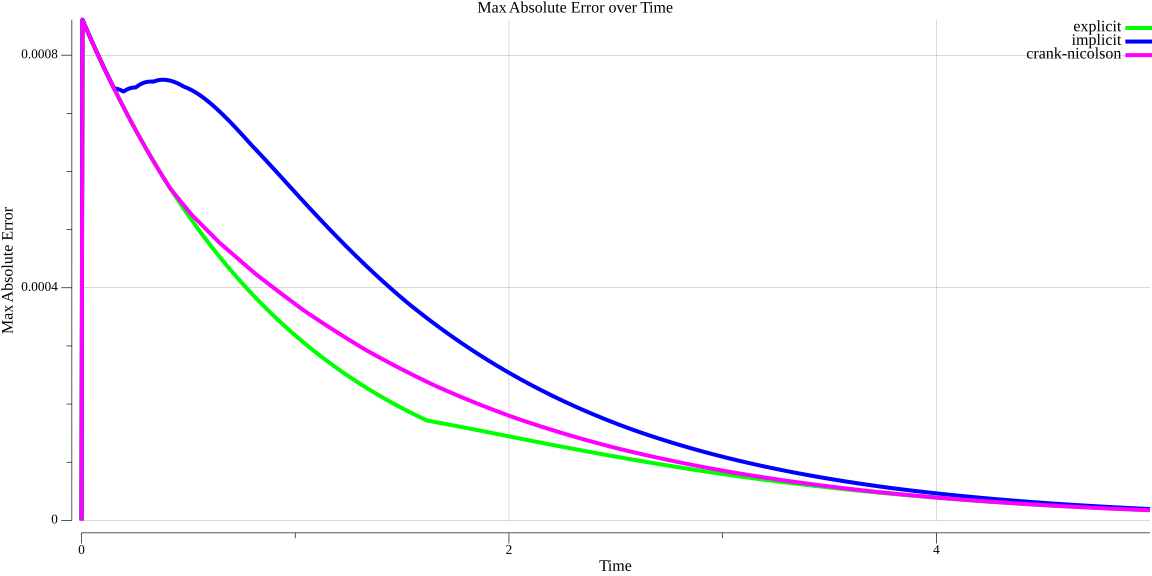
\includegraphics[scale=0.4]{error_plot.png}
\end{center}

\pagebreak
\subsection*{Вывод программы}
\\
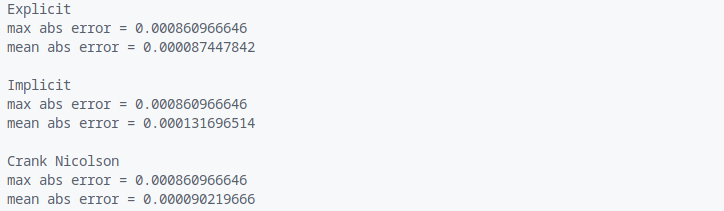
\includegraphics[scale=0.6]{console.png}
\\

\subsection*{Вывод}
Проделав лабораторную работу, я решил начально-краевую задачу для дифференциального уравнения параболического типа тремя различными способами: 
явным, неявным и методом Кранка-Николсона. Проведя сравнение численных решений с аналитическим, я оценил погрешности полученных вычислений. 
Также я визуализировал результаты, что позволило наглядно продемонстрировать динамику изменения температурного поля во времени и пространстве. 
Это дало мне ценное понимание стабильности и точности каждого из применённых методов, а также их пригодность и эффективность для решения задач подобного рода.
\end{document}